\documentclass[acmtog]{acmart}

\usepackage{graphicx}
\usepackage{subfigure}
\usepackage{natbib}
\usepackage{listings}
\usepackage{bm}
\usepackage{amsmath}

\definecolor{blve}{rgb}{0.3372549, 0.61176471, 0.83921569}
\definecolor{gr33n}{rgb}{0.29019608, 0.7372549, 0.64705882}
\makeatletter
\lst@InstallKeywords k{class}{classstyle}\slshape{classstyle}{}ld
\makeatother
\lstset{language=C++,
	basicstyle=\ttfamily,
	keywordstyle=\color{blve}\ttfamily,
	stringstyle=\color{red}\ttfamily,
	commentstyle=\color{magenta}\ttfamily,
	morecomment=[l][\color{magenta}]{\#},
	classstyle = \bfseries\color{gr33n}, 
	tabsize=2
}
\lstset{basicstyle=\ttfamily}

% Title portion
\title{Assignment 1:\\ {Exploring OpenGL and Phong Lighting}} 

\author{Name:\quad  Zhou Shouchen  \\ student number:\ 2021533042
\\email:\quad zhoushch@shanghaitech.edu.cn}
\setlength{\headheight}{25pt}

% Document starts
\begin{document}
\maketitle

\vspace*{2 ex}

\section{Introduction}
In this assignment, the following tasks are finished by using OpenGL.
OpenGL is a state machine, it can remember current status,
modify state according to the input content and state, and can also get the output.

\begin{itemize}
\item Task1: load mesh objects from files
\item Task1: draw the meshes on the screen
\item Task2: phong lighting model with shader on the object
\item Task3: navigation with keyboard and mouse
\item Bonus1: multiple lightning are added on the object
\item Bonus1: use keyboard to change the light styles
\item Bonus2: use geometry shader to draw furry on the bunny
\end{itemize}

\section{Implementation Details}
\subsection{load mesh from file}
At this part, we need to load the mesh into the program.
And we need to load a .obj file from assets document

the .obj document contain three parts
\begin{itemize}
\item \(v\) and followed three float, indicate the position of a vertex
\item \(n\) and followed three float, indicate the normal vector of a vertex
\item \(f\) and followed six float, indicate the index of the three vertices' position and normal vector
\end{itemize}

\subsection{Draw the mesh on the screen}
first we need to load data from file, and we need to define three objects
\begin{itemize}
\item \(VAO\) vertex array object : generate data of vertices
\item \(VBO\) vertex buffer object : send many objects from VAO to GPU, save efficiency
\item \(EBO\)  element buffer object : we can use it to store indices of a trangle to save memory
\end{itemize}
and then we need to generate vertex array, bind VAO;

we also need to generate buffers which bind VBO and EBO:

the \(glEnableVertexAttribArray()\) functions are needed to send the data to the shader
(the position and the normal vector of a vertex)

before using \(glDrawArrays()\) with \(GL\_TRIANGLES\) to draw trangles, bind \(VAO\) to \(VertexArray\) is indispensable.

The most important part to draw the mesh is to write the shaders correctly

\begin{itemize}
\item \(vertex \ shader\)   : recieve the information of vertices such as postion,color,normal vector...
\item \(fragment \ shader\) : pixel the figure and color it
\item \(geometry \ shader\) : input a series of vertices and generate new vertices
\end{itemize}

details:

we use uniform to send data from CPU to GPU, so shader can accept data from code

as for vertex shader, we can use layout(location = 0/1) 0 or 1 and in ... to input data 
such as postion, color, normal vector...
and use out ... to output some processed data to the fragment shader

as for fragment shader, we can use in ... to recieve data from vertex shader
and out ... to output the color to draw the mesh

for this part, the geometry shader is unnesserary, we would use it in the bonus2 to 
draw the normal vectors as the furry on the bunny's surface.

\subsection{phong lightning}
the phong lightning model is combined with three parts,
the ambient, the diffuse, and the specular.

firstly, we need to know the three types of transformation matrix

\(M_{model}\) : transform the local space position into the world space position, original it is identity matrix

\(M_{view}\) : transform the world space position into the view space position, 
we can get the view matrix from the camera paramater

\(M_{projection}\) : transform the view space position into the clip space position, we can calculate it be 
getting the camera's zoom, view aspect, near/far plane by using the function \(glm::perspective\)

and finally, with the local vector \(V_{local}\), we can get the position on screen , the clip vector by using the folloing formula

\(V_{clip} = M_{projection} ⋅ M_{view} ⋅ M_{model} ⋅ V_{local}\)

as for shaders:
\begin{itemize}
\item for vertex shader
we need to in two parameters, the vertex's position and normal vector
we also need to recieve the model, view, projection matrix from the code.

since the position of the certices change by the model matrix \(M_{model}\)
the origin normal vector is no longer vertically to this vertex,
so the normal vector also need to transform
we set an origin edge be T, and it become T' after the \(M_{model}\) transformation,
and the origin normal vector is N, and it become N' after correspondence transformation G

since \(dot(N,T)=0\)and \(dot(N',T')=0\) 

because N'= GN, T'= MT

so  \(dot(N',T')=dot(GN,MT)=(GN)^T(MT)\)

\(=N^TG^TMT=0\)

so  \(G^TM=I\)

so  \(G=(M^{-1})^T=transpose(inverse(M_{model}))\)

so in vertex shader, we need to calculate G, and then use G to transform the origin normal and output the new normal

whats more, since we use a 4-dimension vector to indicate the postion

the vector such as \((x,y,z,w)\) is actually indicate the position \((\frac{x}{w},\frac{y}{w},\frac{z}{w})\)

so if we want to draw the object bigger, we can just set \(w\) a less than 1 constant.


\item for fragment shader

we use fragment shader to output the color.

first we need to recieve the data from vertex shader, to get the vertices' position
and the normal vectors after the transformation

and then we need to work with phong lightning model

it is mainly devided into three parts, each part is one step of the phong lightning model

\begin{itemize}
\item the Ambient Lighting : we need an ambient strenghth to time the light color to get the color on the object
\item the Diffuse Lighting : we use the result dot product to simplize the angle of view dirction and the normal direction,so one important thins is that the vectors we need in the product should be normalized.  
\item Specular Lighting : all vector we needed (view dirction, reflect dirction) should be normal vector
\end{itemize}

and for result color, we just need to sum up all these three kinds of lightning colors.

\end{itemize}
	
\subsection{navigation with keyboard and mouse}

for a camera, we need to store 3 vectors about directions.

They are Front, Right, Up vector.

we need to normalize the vectors, because their length gets closer to 0 the more you look up or down which results in slower movement.

to make the option of navigation easier, we use Euler angle \(Pitch\) and \(Yaw\) to get the front of the camera, and it has the relation of:

\(front.x = cos(Yaw) * cos(Pitch)\)

\(front.y = sin(Pitch)\)

\(front.z = sin(Yaw) * cos(Pitch)\)

\(right = cross(Front, WorldUp)\)

\(up = cross(Right, Front)\)

and the WorldUp vector is generally defined as \((0.0, 1.0, 0.0)\) since the y-axis is pointing to the up.

as for key board control and mouse control, first we need to set up a speed to avoid it moving to fast or slow.
and we need to do modifications by knowing the differences between the last status and current status.

details:
\begin{itemize}
	\item key borad control
	\begin{itemize}
	\item up/down/left/right operation
	move the postion of the camera correspondently.

	\item RGB control operate
	change the status of the RGB dot light.
	\end{itemize}

	\item  mouse control
	\begin{itemize}
	\item the mouse move up/down/left/right
	change the Yaw and Pitch correspondently.
	
	\item if the mouse scroll
	modify the zoom of the camera correspondently.
	\end{itemize}

\end{itemize}

and we need to update the Front, Right, Up vector at anytime.

and for zoom, yaw, pitch, we need to limit their range to avoid the picture changing too much.


\subsection{multiple lightning are added on the object}
for multiple lightning, we just need to calculate each part of the light separately,
with the usage of phong's model, for each light, separately get their ambient, diffuse, specular vector.
in the end, just sum up these things together.

as for the dot light, it is similar with the light in the phong lightning model.
the only modification is that changed thier color from white to RGB, it is easier to control and have a better effect.

one new thing is the spot light with camera.

the part with camera seems eazy, we just need to set the position of the spot light same with the camera's position.

so the important part is how to make a spot light.
its light rays are restricted to a cone shape.
So for a spot light, we need to have a \(coneDirection\) and a \(coneAngle\), with these two paramaters, we can clearly describe a cone.
and for a point, we just need to calculate that whether it is in the range of the spot light.
if not, just set the \(intensity \) be 0, so that the light will not have any effect on it.

for convenience, we can use the \(clamp\) function, to range the \(intensity \) between \([0,1]\)
in the last, the ambient, diffuse, specular should time attenuation and intensity.

\subsection{use keyboard to change the light styles}
since we have finished the last part, put multiple lightning on the object,
this part is just do some modifications.

we can set some variables, each time we tap the keyboard, the variable change 
between 0 and 1, and we can just let the variable times the result vector,
 so we can change to put on the light(variable=1) or not(variable=0)

\subsection{use geometry shader to draw furry on the bunny}
As we know, the geometry shader can recieve data from vertex shader, and then
generate new set of vertices.

first we need to change the original vertex shader, to \(vs_out\) to output the normal vector

and then in geometry shader, we need to recieve from the vertex shader,
 after that, we can set a magnitude, that symbolize the length of the vector we want to draw.

say it concretely, we draw a line which start at the vertex's position, with the 
direction of its normal vector, draw the length of magnitude.

With all vertices have this option, it seems that we draw the fur on the bunny's surfacce.


\section{Results}
the results can be seen in the pictures.

\begin{itemize}
\item Fig. 1. 
As it is shown in  We can observe the bunny from different directions with the navigation
by using the keyboard and mouse with phong lightning.

The first four pictures are from the different direction, and the last two pictures are with zoom.

\item Fig.2. we use the spot-light with camera, so no matter how we move the camera
the part front of us is always light up. So we can clearly see the bunny from all directions. As the third picture, compared with single 
phone lightning, we can clearly see the buttom of the bunny. 

\item Fig.3. based on the sopt-light with camera, we can put some other light from different positions and directions.
as it is said in \(section 2.6\) we can tap the kep board to open the red/green/blue
lights. The multiple lights(spot light, direction lights with different colors) on the bunny are shown in the figure.
 
\item Fig.4. we use geometry shader to draw the normal vector of each vertex, and set the color
of the vector be brown, to make it have the effect of fur. 

\end{itemize}

\begin{figure}[h]
	\centering
	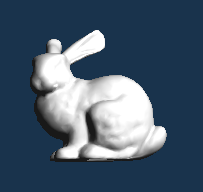
\includegraphics[width=4cm,height=5cm]{1}
	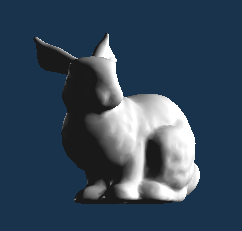
\includegraphics[width=4cm,height=5cm]{2}
	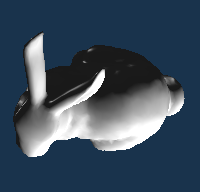
\includegraphics[width=4cm,height=5cm]{3}
	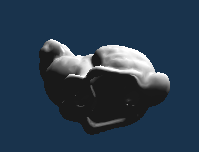
\includegraphics[width=4cm,height=5cm]{4}
	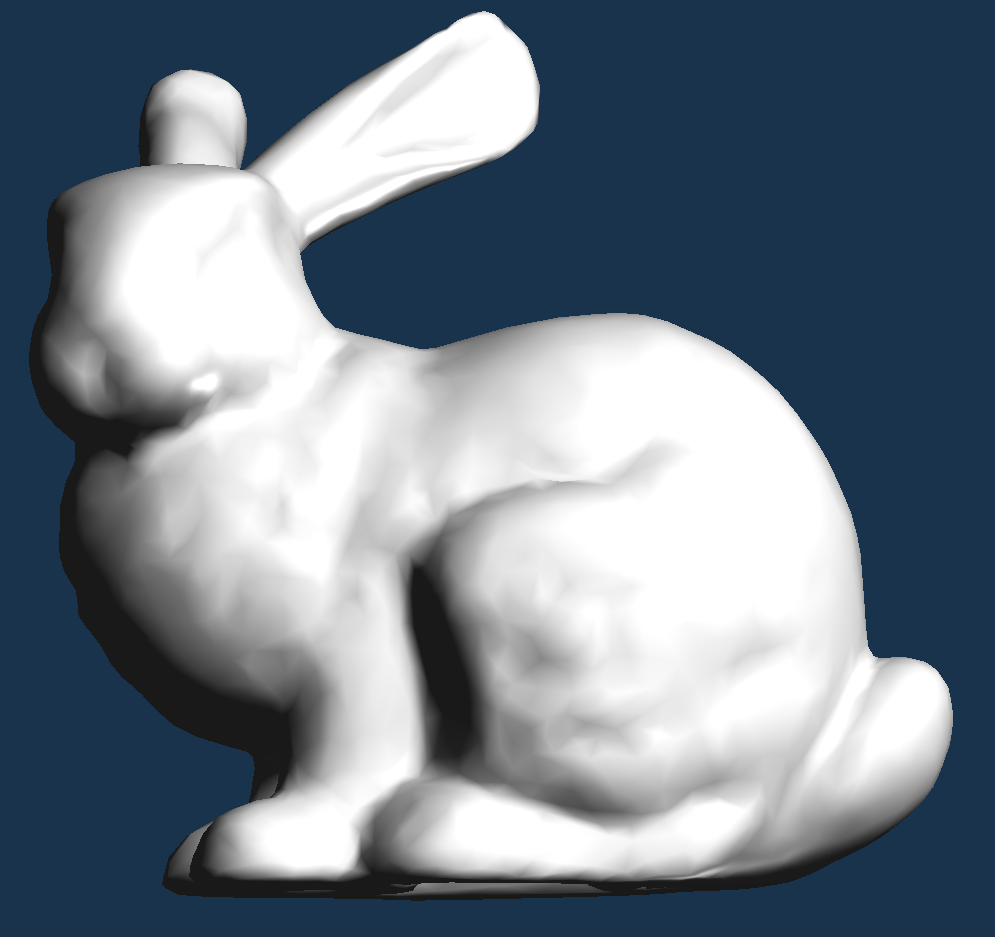
\includegraphics[width=4cm,height=5cm]{5}
	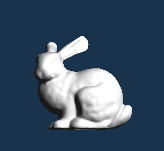
\includegraphics[width=4cm,height=5cm]{6}
	\caption{phong lightning with navigation}
\end{figure}

\begin{figure}[h]
	\centering
	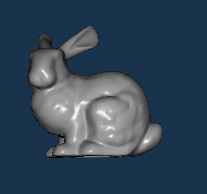
\includegraphics[width=4cm,height=5cm]{7}
	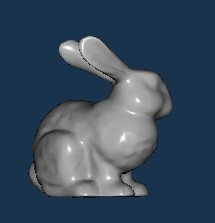
\includegraphics[width=4cm,height=5cm]{8}
	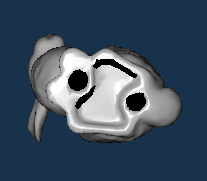
\includegraphics[width=4cm,height=5cm]{9}
	\caption{spot-lightning with navigation}
\end{figure}

\begin{figure}[h]
	\centering
	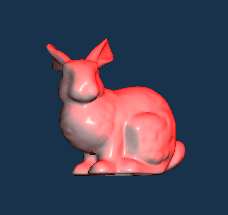
\includegraphics[width=4cm,height=5cm]{r}
	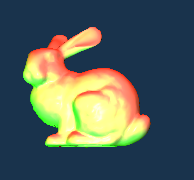
\includegraphics[width=4cm,height=5cm]{r+b}
	\caption{spot light with camera and multiple lightning}
\end{figure}

\begin{figure}[h]
	\centering
	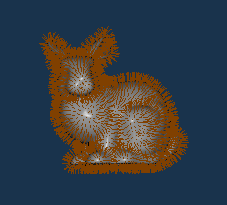
\includegraphics[width=4cm,height=5cm]{ugly}
	\caption{geometry shader make fur for the bunny}
\end{figure}
.
\\
\end{document}
